\clearpage
\title{Problem 4.1}
\author{}
\date{}
\maketitle

\section*{Problem Description}
Write a code to take input from user as Binary and output it as Binary.

\section*{Tools Used}
\begin{itemize}
    \item emu8086 - 8086 Microprocessor Emulator
    \item MacTeX -\LaTeX  compiler.
    \item VS Code with \LaTeX workshop extension as a text editor.
\end{itemize}

\section*{Process}
\subsection*{Code:}

\begin{multicols}{2}{|}
    \begin{minted}[linenos,breaklines,breakanywhere]{nasm}
DATA SEGMENT
    CR EQU 0DH
    LF EQU 0AH
    CNT DB 17
DATA ENDS

CODE SEGMENT 
    ASSUME CS: CODE, DS: DATA
    
START:
    MOV AX, DATA
    MOV DS, AX
    
    XOR BX, BX
    MOV CX, 16
    
    MOV AH, 1
    INT 21H
    
INPUT:
    CMP AL, 0DH
    JE EXIT
    
    AND AL, 0FH
    SHL BX, 1
    OR BL, AL
    
    INT 21H
    
    JMP INPUT

EXIT: 
    MOV DL, CR
    MOV AH, 2
    INT 21H
    MOV DL, LF
    INT 21H
    
PRINT:
    DEC CNT
    JZ END_
        
    RCL BX, 1
    JC PRINT1
    JNC PRINT0
    
PRINT1:
    MOV DL, '1'
    MOV AH, 2
    INT 21H
    
    JMP PRINT
    
PRINT0:
    MOV DL, '0'
    MOV AH, 2
    INT 21H
    
    JMP PRINT

END_:
    MOV AH, 4CH
    INT 21H    
        
CODE ENDS
END START
    \end{minted}
\end{multicols}


\subsection*{Output}
\begin{center}
    \centering
    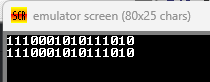
\includegraphics[width = .4\textwidth]{BIN.png}
    \captionof{figure}{Binary input \& output}
\end{center}

